\renewcommand{\thesubsection}{\textcolor{red}{\Roman{section}.\arabic{subsection}}}
\renewcommand{\thesubsubsection}{\textcolor{red}{\Roman{section}.\arabic{subsection}.\alph{subsubsection}}}

\setcounter{section}{0}
\sndEnTeteCoursDeux

\begin{mdframed}[style=titr, leftmargin=60pt, rightmargin=60pt, innertopmargin=7pt, innerbottommargin=7pt, innerrightmargin=8pt, innerleftmargin=8pt]

\begin{center}
\large{\textbf{Chapitre 2 : Les solutions acqueuses}}
\end{center}
\end{mdframed}
Dans ce chapitre, nous nous intéressons à un type de mélange en particulier : les solutions acqueuses.

\begin{tcolorbox}[colback=blue!5!white,colframe=blue!75!black,title=Mots clés du chapitre :]
Solution, solvant, soluté, dissolution, solubilité, 
\end{tcolorbox}


\section{Composition d'une solution}
\begin{Large}
    \ding{43}
\end{Large}\textit{Voir activité 1 : Concentration en masse}
\subsection{Définitions}
\begin{tcolorbox}[colback=green!5!white,colframe=green!75!black,title=\textbf{Solution, solvant, soluté}]
\begin{center}
    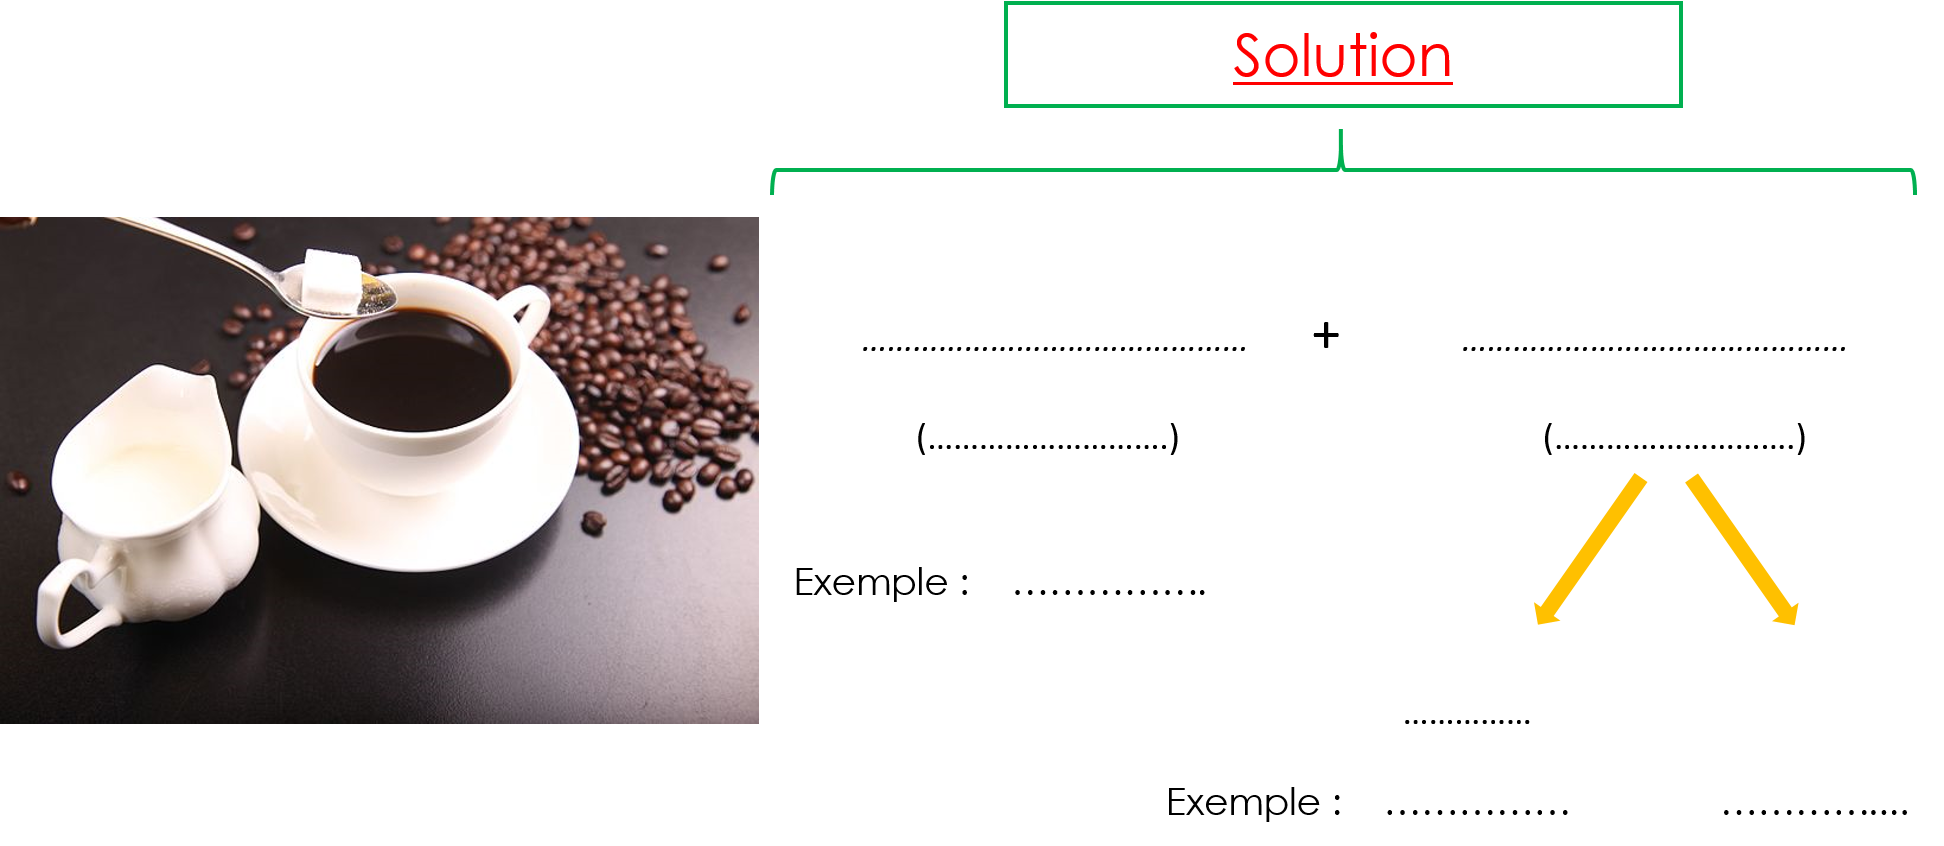
\includegraphics[width=\textwidth]{Images/Chapitre_2/Solution_def.png}
\end{center}
\end{tcolorbox}
Sur l'image de la tasse de café ci-dessus, qui jouent le rôle du solvant et des solutés ? Comment s'appelle la solution ?\\
\textit{Réponse :} \gap{........................................................................................................................}\\

\begin{Large}
    \ding{45}
\end{Large}\textbf{Exercice DOC : l'alcool dénaturé.}

\section{La solubilité}

\begin{tcolorbox}[colback=green!5!white,colframe=green!75!black,title=\textbf{Définition de la solubilité}]
La solubilité, notée $s$, d'une espèce chimique est la masse maximale de cette espèce que l'on peut dissoudre dans $1$~L de solvant. Elle s'exprime en $\mathbf{g.L^{-1}}$.\\
Il s'agit d'une \textbf{concentration massique} !
\end{tcolorbox}

\section{La concentration en masse}

\section{Préparer des solutions}

\subsection{La dilution}

